\chapter{Analysis}

\section{Introduction}
	My client is a local church based in central Cambridge, they currently have a pen, paper and verbal system for organising many of the staff,
	assets and events within the church. There is also no official way to report incidents both pastoral and material.

\subsection{Client Identification}
	My client is a mid-sized city centre church with 250 regular attendees and around 60 people who are involved in rotas and with responsibilities.
	There are several components to the Church's operation broadly split into two sections: People and resources. People represents all of the meetings, appointments and responsibilities, it also includes records of these meetings and appointments; and resources represents the materials that are required for the smooth operation of the Church, for example Teabags and Support Tickets. The Church also needs to regularly send out emails to inform it's members of their responsibilities and to keep them up to date with church news.

	They use a mixture of Apple iMac and Windows machines, so it's essential that any software they use is cross-compatible and doesn't use any OS spec
	ific features while also supporting all the quirks within a particular OS. The church also has a central server and networking capabilities which they use for filesharing and remote access of devices such as projectors.

	The Church relies heavily on being properly organised, which places a large amount of responsibility and pressure on the office administrator and
	staff team. Many of these tasks can be automated, however there are no automatic systems in place. Also because the Church leadership is elected and the people holding the various roles change regularly, ofteh confusion emerges during transition periods.

%TODO: identify the individuals within the organisation more clearly - job roles??
%TODO: Elaborate on the staff team and job roles.

\subsection{Define the current system}
	The current system is a mixture of word of mouth and emails containing scraps of information. It consists of three main elements: the meetings, duties
	and appointments part of the system, the support tickets and referrals system and the stock management system (this includes cafe resources, office
	stationary and anything that has to be purcheased regularly or has a supply which can be depleted). Currently, people are expected to keep
	and duties in whatever diary system they have and they do this with a reasonable degree of success. For the cafe stock management, whoever
	is operating the till keeps a handwritten record of whatever has been sold, which is then added to a central ledger at the end of the day.
	For all of the incident reporting (support tickets, prayer requests etc) emails are used as the primary way of official communication, often
	the same set of people are copied into whatever email conversations that take place. For membership inormation, handwritten record cards
	containing all of the information for each member are stored and archived in two locations.

\subsection{Describe the problems}
%problems:
%	no official reminders of duties and appointments
	The current system does not send out centralized reminders for people who have duties and/or meetings, people are expected to remember their
	own meetings. This adds potential for people to forget about meetings and duties, especially when they're organised months in advance
%	potential for omissions, limitations in terms of scalability
	The system for dealing with stock management in the cafe adds potential for omissions, the often elderly people responsible for this aspect
	often forget to write things down and sometimes find it quite difficult to use the old and complex till system. Also all of the orders have
	to be cross-referenced with a daily price list and any offers or deals are factored in, this adds further potential for error and could mean
	that the cafe will loose money. The lack of comprehensive records means that the cafe will have trouble accurately guaging trends in the
	customers and fail to adapt to these trends.
%	no centralised, secure or official record.
	Because a lot of the pastoral information that has to be communicated to people in various positions around the church is strictly
	confidential, email is not a bad choice, however it does not provide a centralised set of records which would be required to ensure
	professional and caring conduct. So the current system fails to ensure that if any official communication is called into question
	that there is an official, untampered record of it.
%	no synchronisation/potential for omissions, data protection act states that only appropriate and up to date information is stored - these record cards do not meet these standards.
	The data protection act states that information about anyome must not be kept any longer than necessary, and it must be kept up
	to date, some of these record cards date back to the 1920s and contain information about people who no longer attend the church
	and people who are deceased, there is no easy way to update these record cards and there are no failsafes the ensure their validity
	and their complience with the DPA.

\subsection{Section appendix}

\section{Investigation}

\subsection{The current system}

\subsubsection{Data sources and destinations}
Because the Church relies on information being shared between different people with different responsibilities, this information has to move between people.

\begin{landscape}

    \begin{table}
    \centering
    \caption{My caption}
    \label{my-label}
    \begin{tabular}{llll}
    \hline
    \multicolumn{1}{|l|}{Source}             & \multicolumn{1}{l|}{Data}                     & \multicolumn{1}{l|}{Example}                                                                         & \multicolumn{1}{l|}{Destination}                       \\ \hline
    \multicolumn{1}{|l|}{Member}             & \multicolumn{1}{l|}{Name and Contact details} & \multicolumn{1}{l|}{John Smith, jsmith@mailmailmail.com}                                             & \multicolumn{1}{l|}{Membership Records}                \\ \hline
    \multicolumn{1}{|l|}{Appointment}        & \multicolumn{1}{l|}{Who, what when and where} & \multicolumn{1}{l|}{John smith, pastoral visit, 10:30 Thursday  4th Oct 2013, Church Meeting room 4} & \multicolumn{1}{l|}{Attendee's Diaries}                \\ \hline
    \multicolumn{1}{|l|}{Referral Ticket}    & \multicolumn{1}{l|}{Who and what}             & \multicolumn{1}{l|}{John Smith, Prayer Request for his niece's hospital visit}                       & \multicolumn{1}{l|}{Prayer Team's records}             \\ \hline
    \multicolumn{1}{|l|}{Support ticket}     & \multicolumn{1}{l|}{What and when}            & \multicolumn{1}{l|}{Faulty Microphone, Sunday xth of January.}                                       & \multicolumn{1}{l|}{Finance Team's \'to purchase\' list} \\ \hline
    \multicolumn{1}{|l|}{Cafe Order}         & \multicolumn{1}{l|}{What, when and how much}  & \multicolumn{1}{l|}{2x cup of tea, Thursday 4th Oct 2015, £3.65}                                     & \multicolumn{1}{l|}{Cafe Management's ledger}          \\ \hline
    \multicolumn{1}{|l|}{Resources Purchase} & \multicolumn{1}{l|}{What, when and how much}  & \multicolumn{1}{l|}{3x replacement microphone, 4x AA batteries; Wednesday 3rd Oct 2015, £215.30}     & \multicolumn{1}{l|}{Finance Team's ledger}             \\ \hline
    \multicolumn{1}{|l|}{}                   & \multicolumn{1}{l|}{}                         & \multicolumn{1}{l|}{}                                                                                & \multicolumn{1}{l|}{}                                  \\ \hline

    \end{tabular}
    \end{table}
\end{landscape}


\subsubsection{Algorithms}
 The current system uses few algorithms for it's operations, for the current system doesn't actually do anything, it simply tells people to do things.
For Pastoral or Support tickets:
\begin{algorithm}[H]
	\caption{Support Referral request:}
	\begin{algorithmic}[1]
		\RECEIVE{$The problem$}
		\Repeat
			\RECEIVE{$Is the problem solved?$}
		\Until{$Problem is solved$}
	\end{algorithmic}
\end{algorithm}

And for the resources stock management:
\begin{algorithm}[H]
	\caption{Stock management algorithm}
	\begin{algorithmic}[1]
		\RECEIVE{$The minimum safe amount of this resource$}
		\RECEIVE{$The cost of this item$}
		\RECEIVE{$The current amount of this resource$}
		\If{$The current amount of the resources \textless minumum required amount of this resource$}
			\SEND{$Buy more of this resource$}
		\EndIf
	\end{algorithmic}
\end{algorithm}

\subsubsection{Data flow diagram}

\begin{figure}[H]
	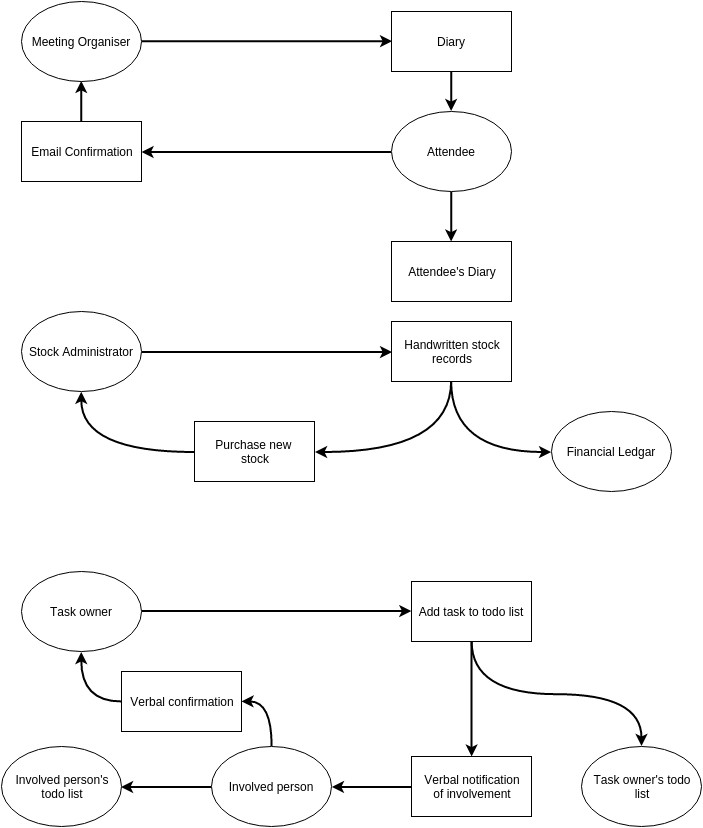
\includegraphics[width=\textwidth]{./Analysis/diagrams/dfc.jpg}
\end{figure}

\subsubsection{Input Forms, Output Forms, Report Formats}

The current system for meeting arrangement has one input form: that is the written entries in diaries. These contain the date,
 time, location of the meeting and a breif description of what the meeting is concerning. These forms are stored in the personal
 diary belonging to the meeting's owner.

If the meeting has more than one attendee, then the meeting owner will email the attendees requesting that they attend and their
 reply will be a form of input into the meeting event.

For the subsystem managing the staff team's tasks, these are usually a handwritten note handed from one member of staff to another.
 Members of staff often form a compiled list of tasks for that day as a report format. These are often handwritten and do not follow a set style.

\begin{figure}[H]
	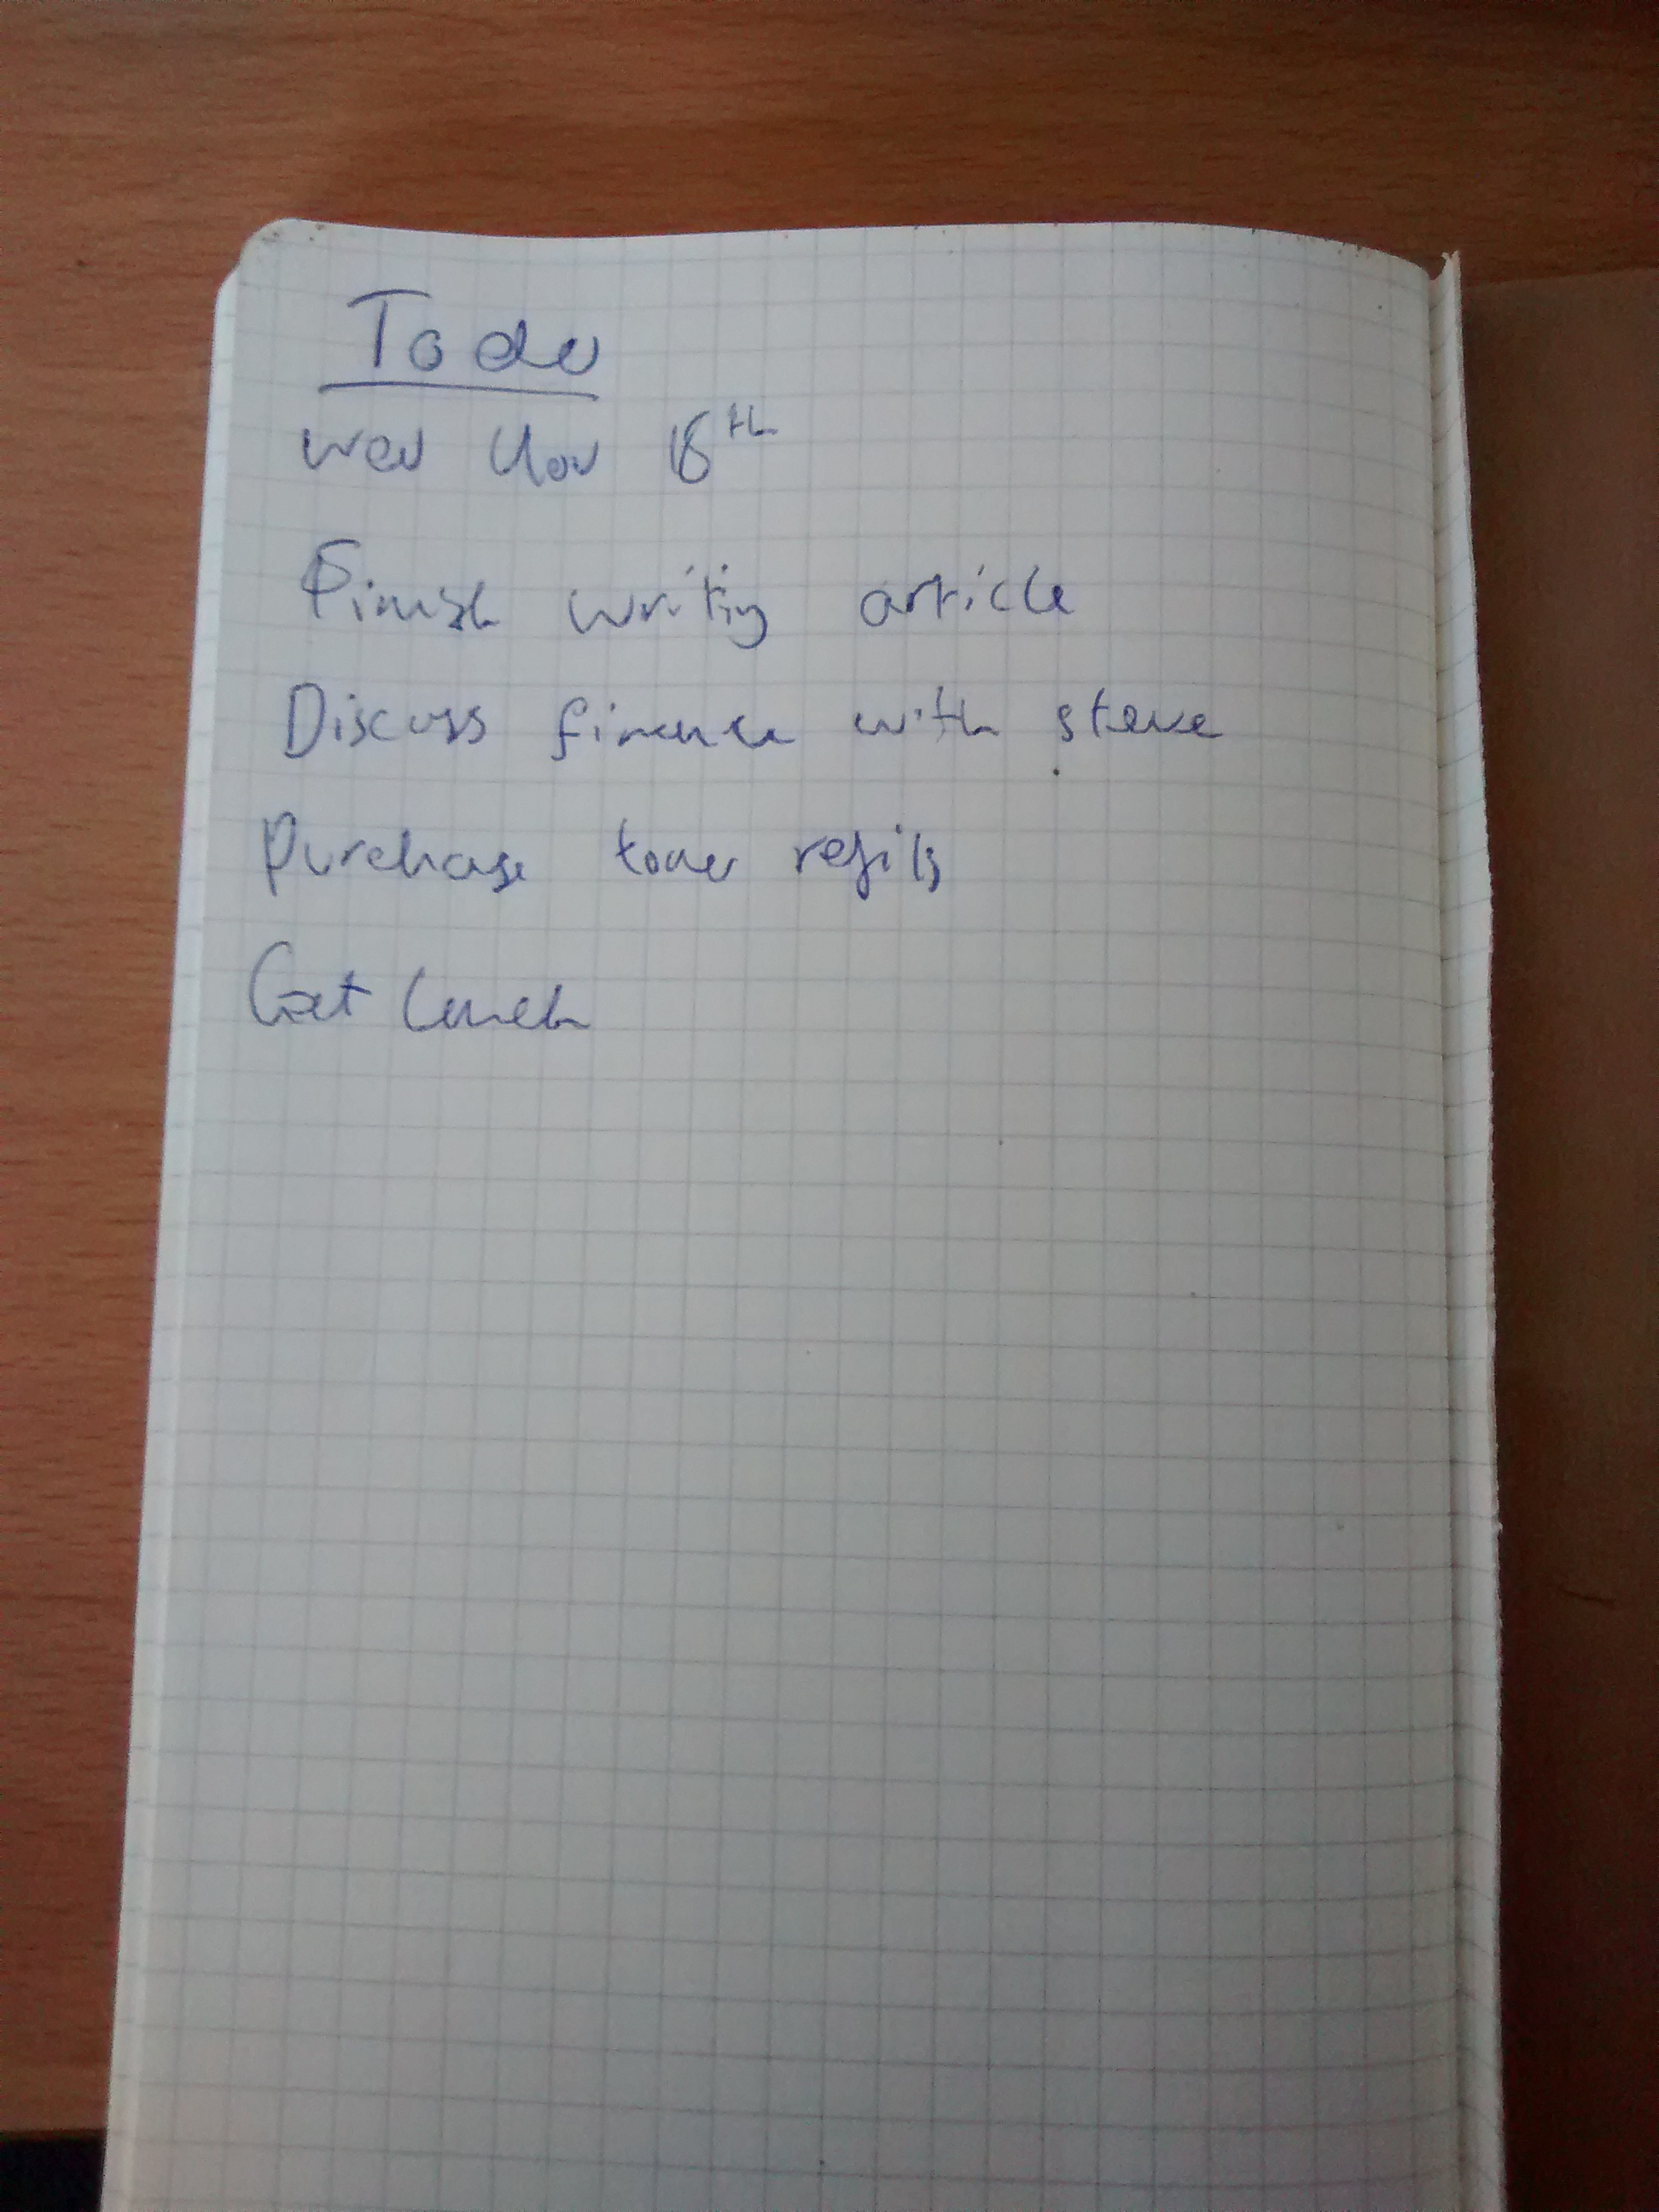
\includegraphics[width=\textwidth]{./Analysis/diagrams/todo.jpg}
\end{figure}

The current system for managing resources uses input from recipts taken from the till in the cafe and from handwritten notes from
other departments within the Church detailing expendature and requesting resources. The output from this system is in the form of a handwritten ledgar maintained by the Church administrator.

\subsection{The proposed system}

\subsubsection{Data sources and destinations}

\begin{table}[]
\centering
\label{my-label}
\begin{tabular}{|l|l|l|l|l|}
\hline
Source & Data & Type & Max Size & Destination \\ \hline
Meeting Owner & Attendees & List of Integer UserIDs & 1024 Bytes & Database - Meetings \\ \hline
Meeting Owner & Meeting title & String & 255 bytes & Database - Meetings \\ \hline
Meeting Owner & Meeting Location & String & 512 Bytes & Database - Meetings \\ \hline
Meeting Owner & Meeting Time & String & 18-24 Bytes & Database - Meetings \\ \hline
Meeting Attendee & Confirm Attendance & Boolean & 1 Byte & Meeting Owner \\ \hline
Task Creator & Task Title & String & 50 Bytes & Database - Task Records \\ \hline
Task Creator & Task Description & String & 4 KiB & Database - Task Records \\ \hline
Task Creator & Related People & Lister of Integer UserIDs & 1024 Bytes & Database - Task Records \\ \hline
Person & Username & String & 255 Bytes & Database - Users \\ \hline
Person & Real Name - Firstname & String & 255 Bytes & Database - Users \\ \hline
Person & Real Name - Lastname & String & 255 Bytes & Database - Users \\ \hline
Person & Password hash & String & 32 Bytes & Database - Users \\ \hline
Administrator & User Permissions & Integer & 1 Byte & Database - Users \\ \hline
Resource Manager & Resource Title & String & 255 Bytes & Database - Resources \\ \hline
Resource Manager & Resource Cost & Integer & 4 Bytes & Database - Resources \\ \hline
Resource Manager & Current Resource Quantity & Integer & 4 Bytes & Database - Resources \\ \hline
Resource Manager & Required Resource Quantity & Integer & 4  Bytes & Database - Resources \\ \hline
Resource Maneger & Person With Responsibility & Integer (ID) & 4 Bytes & Database - Resources \\ \hline
Resource Management Process & Understocked Resources & Integer (ID) & 4 Bytes & Database - Understocked Resources \\ \hline
Resource Management Process & Understocked Resources notification & Integer (ID) & 4 Bytes & Database - Tasks \\ \hline
Meeting Notification Process & NewMeetingID & Integer (ID) & 4 Bytes & Database - UserMeeting \\ \hline
 &  &  &  &  \\ \hline
 &  &  &  &  \\ \hline
\end{tabular}
\end{table}

\subsubsection{Data flow diagram}

\begin{figure}[H]
	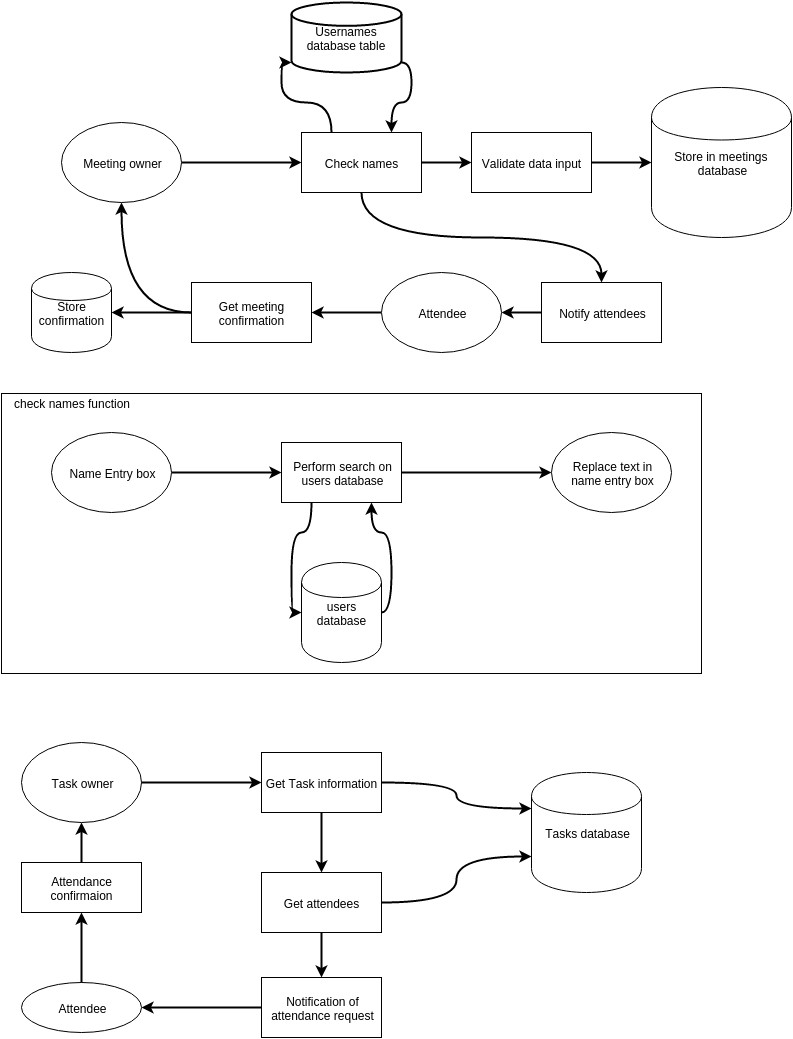
\includegraphics[width=\textwidth]{./Analysis/diagrams/dfp1.jpg}
\end{figure}
\begin{figure}[H]
	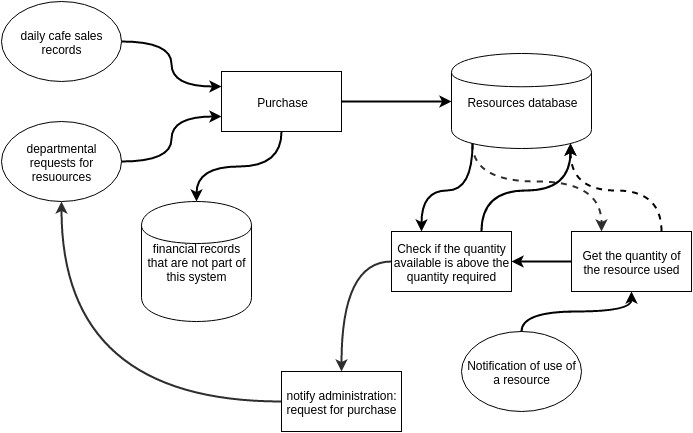
\includegraphics[width=\textwidth]{./Analysis/diagrams/dfp2.jpg}
\end{figure}

\subsubsection{Volumetrics}
	% The church has between 150 and 250 congregates meeting every week, of these congregates there are about 50 \'members\'. In the Baptist
	%Church, a member is defined as someone who attends regularly enough and is commited to both Christianity and the Church who is able to
	make proposals and cast votes in the monthly Church administration meeting. This means that the scale of the databases required for staff
	management will not be huge. However, for the meetings management elements of the system, there is not a limit to the number of meetings
	and appointments that will be organised therfore this part of the system must be scaleable infinitely, or to the capacity of the current
	hardware. The support and referral ticket system also must be able to scale to the needs of the congregation, it also needs to have an
	archive of past events.
	% \\
	% The entire system has to be able to account for large-scale events, for example the Church acquiring another building, if the
	branches out into Church plants or if the Church joins a union of Churches, therfore within the system there should be a way o
	f managing more than one separate church.

	There are 5 members of the staff team which will have between 2 and 5 meetings per day, which means in one month, the system will
	have up to 750 meetings, eacho of which will require up to 1815 Bytes, which will total at 1.3MiB per month for the meetings system.
	However, the number of people who will be involved in meetings will be subject to change on a weekly basis, it could easily double,
	triple or more which means that this part of the database could use up to 5MiB per month and up to 60MiB per year.

	The user's table will contain a record of each user who has meetings, which totals at 798 Bytes per person. In a large city
	centre Church, there are approximately 250 congregates, of which 50 will be involved with meetings, which means the user's
	database will require at minumum, 39KiB. However this number is subject to change and could easily double in the space of a year,
	but because of the data protection act, some means of ensuring the data does not expire would mean that as, or shortly after new users
	are added, the old users are removed so the size of the table will only fluctuate by $\pm$10KiB, so to ensure there's alway enough space,
	this table will be allocated 60KiB.

	The tasks table, which is effectively a record of each user's todo list, will contain records for between 5 and 10 users each with up
	to and estimated 15 items per day. Each item is 5170 Bytes, which means every day, each user will generate up to 76Kib, with up to 10
	users totalling at 760Kib, so in a month the database will contain up to 22.8Mib. However, the nature of the tasks means that they will
	expire after a certain amount of time, which will limit the size of the database. If the expiry period of each task is set to one year,
	this table will not exceed 273.6Mib

	The resources table will contain a record of all of the things the Church regularly buys, including cleaning supplies, food, drinks,
	cafe supplies. The church has several areas which require resources, some of which require more than others. If in total, the Church
	buys 300 consumeable products, each record will require 271 Bytes, with 300 items, the table will require 80KiB, however there is potential
	for new items to be added on a regular basis, so this table could easily grow to 100KiB.

	The total database requirements are 334MiB, for a year's worth of data. The program itself, the PyQt Library and Python will
	require about 130Mib, which means the total estimated size of the system will be 464MiB.


\section{Objectives}

\subsection{General Objectives}
	The client needs software to manage people and their appointments, the pastoral and support events and the material resources for the
	various aspects and functions within the Church. The entirity of the system needs to be useable by anyone who could potentially be included
	in a rota, however the system should not require a great deal of training and should be self explainitory if possible.
	%Gonna need more detail here


\subsection{Specific Objectives}
	%do a lovely itemize thing
	The system must...
	\begin{itemize}
		\item Contain and manage a complete record of all past, present and furute dealings the Church has, this includes and is not limited to purchases, support/referral tickets and staff meetings.
		\begin{itemize}
				\item A central list of Past and future meetings, accessable to administrators.
		\end{itemize}
		\item The system must also remind people concerned with these meetings.
		\begin{itemize}
				\item A central hub which displays pending notifications in a clear way.
		\end{itemize}
		\item The system must keep all of these records securely and in accordance to the Data Protection act.
		\begin{itemize}
			\item The system must use encryption to secure the data.
			\item The system must also have a level of user access control.
		\end{itemize}
		\item The system must be easy to use, and have a way of providing help for every little feature as it is to be used by people with little or no training and/or computer experience.
		\begin{itemize}
			\item The system must have a minimal control interface without excessive functions
			\item All buttons and actions must be labelled clearly
			\item All written content must be in easily understandable standard english without technical terms.
		\end{itemize}
		\item The system has to be synchronised with a central service to ensure no omissions of information due to syncronisation errors.
	\end{itemize}

\subsection{Core Objectives}
	\begin{itemize}
		\item Complete record of all official meetings.
		\item UI which informs users of their pending tasks.
		\item Easy to use
		\item Security of data
	\end{itemize}

\subsection{Other Objectives}
	\begin{itemize}
		\item Google Maps integration for meetings
		\item Email alerts for tasks/meetings
	\end{itemize}

\section{ER Diagrams and Descriptions}

\subsection{ER Diagram}

\begin{figure}[H]
	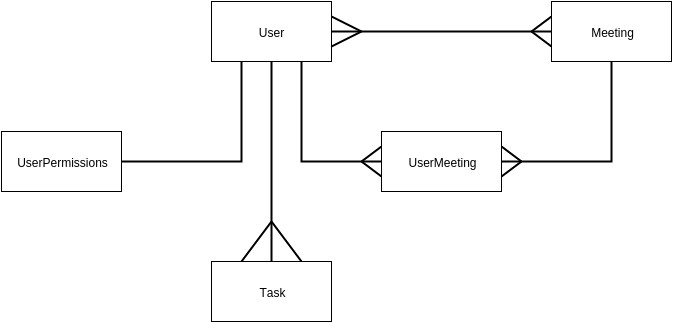
\includegraphics[width=\textwidth]{./Analysis/diagrams/era.jpg}
\end{figure}

\subsection{Entity Descriptions}

User(\underline{UserID}, UserFirstname, UserLastname, UserPasswordHash, Permissions)

Meeting(\underline{MeetingID}, MeetingOwner, MeetingTitle, MeetingDateTime, MeetingPlace, MeetingAttendees)

MeetingAttendee(\underline{UserID}, \underline{MeetingID}, UserMeetingConfirmation)

Task(\underline{TaskID}, TaskTitle, TaskDescription, TaskOwner, TaskAttendees, TaskExpiry, Priority)

TaskAttendee(\underline{TaskID}, \underline{UserID}, UserTaskConfirmation)

Resource(\underline{ResourceID}, ResourceName, ResourceCost, ResourceQuantity, ResourceRequiredQuantity)

\subsection{Data dictionary}

%TODO: this is a table containing the names, types and sizes of each item

\section{Object Analysis}

\subsection{Object Listing}

\begin{itemize}
	\item User
	\item Attendee
	\item Meeting
	\item Task
	\item Resource
	\item Event
\end{itemize}

\subsection{Relationship diagrams}

\begin{figure}[H]
	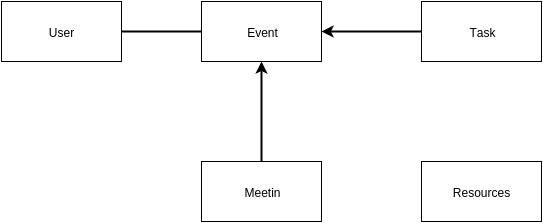
\includegraphics[width=\textwidth]{./Analysis/diagrams/orld.jpg}
\end{figure}

\subsection{Class definitions}

\begin{figure}[H]
	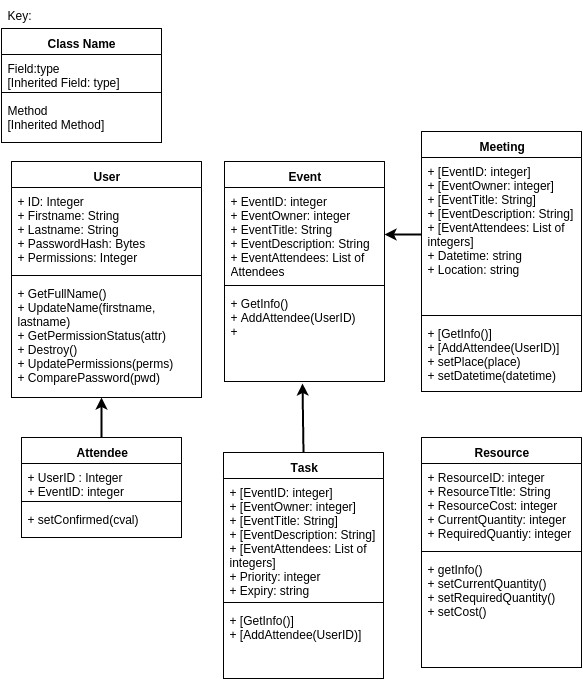
\includegraphics[width=\textwidth]{./Analysis/diagrams/ods.jpg}
\end{figure}

\section{Other Abstractions and Graphs}

\section{Constraints}

\subsection{Hardware}

	The Church currently uses a variety of aging PCs and Apple Macs, therfore the software cannot use any OS dependant resources.
	\\The proposed system does not require any high performance computing systems, nor does it require a large amount of storage.
	\\The lowest spec PC running on the system is:
	\begin{itemize}
		\item Intel Pentium, 2.13GHz \(mid 2009\)
		\item 2 GiB ram
		\item 100Mbit NIC
		\item 17\" 4:3 Monitor
		\item 250Gb HDD
	\end{itemize}
	These specs are more than enough for handling all of the processing and GUI elements of the program, the user may experince slight delays
	during database queries, especially if the database becomes large (after one or two years, without the automatic clearing process), but these
	shouldn't last more than a few seconds. This necessitates processes to automatically manage expired data.


	The system UI will need to be able to scale for smaller screen sizes to ensure all of the required controls and information are on screen at one time.


\subsection{Software}
	Because the computers which will run this system are running both OS X and Windows, the system cannot depend on OS specific resources or quirks,
	and the system must be self contanied. The people operating the system might have little or no training or experice with using computers, which
	means the system must contain comprehensive and simple documentation both on paper and included in the system.

\subsection{Time}
	The only time constraint for this project is (unless changed) January 2016, this is set by the College. Because the proposed system will replace
	an existing system, there is less time pressure from the client as they are able to continue operating, albeit at a reduced rate, without the proposed system.

\subsection{User Knowledge}
	The proposed system will be used by several people, all with different ages and with different amounts of experience in ICT systems so it is necessary
	to assume no knowledge when designing the UI and the documentation.

\subsection{Access restrictions}
	The information processed by this system is often confidential, so the proposed system includes encryption and user access control, with
	authentication by password. The system adminstrator is able to change the access privelliges of each of the users

\section{Limitations}

\subsection{Areas which will not be included in computerisation}
		%TODO: Do this bit!!!

\subsection{Areas considered for future computerisation}
	An extension to the system could be developed to replace the checkout element of the cafe which would automatically update resources and
	it would be able to keep financial records and report them to the cafe management on a regular basis, this would completely cut out the time
	required to input the updates to the sales information at the end of the day, and it would give the management live insights into
	the operation of the cafe.

\section{Solutions}

\subsection{Alternative solutions}

\begin{table}[]
\centering
\caption{My caption}
\label{my-label}
\begin{tabular}{|l|l|l|}
\hline
Solution                       & Advantage                                                                                                                                                                                                                                                                     & Disadvantages                                                                                                                                                                                                                                              \\ \hline
Custom set of spreadsheets     & Does not require bespoke software                                                                                                                                                                                                                                             & does not store data securely, does not organise data, difficult to share information between people. No support for notifications                                                                                                                          \\ \hline
\"Webapp\"                       & Cloud resource, accessible anywhere from any device, offsite backups \& server resources. Support can be issued remotely                                                                                                                                                      & Has a regular service charge, a web based application is open to everyone in the world therefore the application must be secure.                                                                                                                           \\ \hline
Revising the current system    & Very low cost, no external contractors required, no need to retrain and/or learn new skills.                                                                                                                                                                                  & All of the current problems will still exist, management of data becomes a manual and laborious task.                                                                                                                                                      \\ \hline
Command Line application (CLA) & Quicker and easier to program, most storage and processing efficient solution                                                                                                                                                                                                 & Requires significant training and documentation. Most of the users working for the client have little or no computer experience therefore a command line application would be completely foreign to them and would probably scare them away from using it. \\ \hline
Desktop application with GUI   & Can be written in Python so all of the core code will be the same as in a CLA, except it will have a GUI to
operate those functions. Layout can be easy to use and can include easy to reach help at every point of entry. Could be used with a touch screen for ease of use. & GUIs are more time consuming to program than CLAs as the layout of the UI requires significant design process. Also rendering and operating GUI requires more processing than a CLA.                                                                       \\ \hline
\end{tabular}
\end{table}

\subsection{Justification of chosen solution}

% I have chosen to use a Python Desktopp GUI app for the following reasos:
\begin{itemize}
	\item The application will meet my client's specific needs in a user friendly way that cannot accidentally be changed, unlike a spreadsheet
	\item The digital storage of the user's data will fit on existing hardware.
	\item All the data contained in the database can be easily backed up and restored.
	\item The GUI has all of the advanced features of the CLA but they are more easily accessable.
	\item The python language has a balance programming simplicity and computing versitility that make it perfect applications such as these, when there's a relatively small time frame but the task requires some advanced features.

\end{itemize}
